\chapter*{instalasi}


\section*{\textit{ Instalasi Python 3}}
\begin{enumerate}
		\item Clik apk anaconda lau clik install. Selanjutnya clik next.
		\begin{figure}[h]
			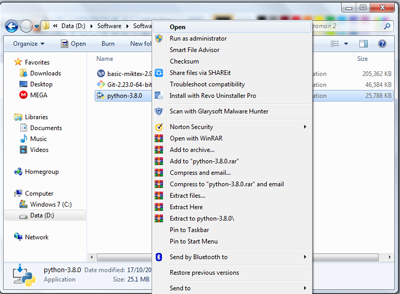
\includegraphics[width=4cm]{figure/1.png}
			\centering
			\caption{install anaconda}
			\end{figure}
		\item Selanjutnya , clik I agree.
			\begin{figure}[h]
			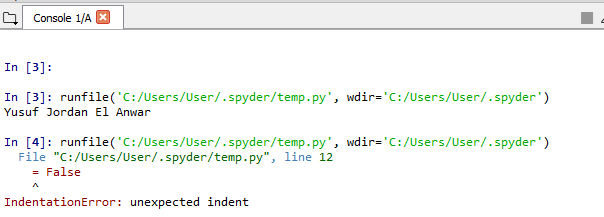
\includegraphics[width=4cm]{figure/2.png}
			\centering
			\caption{licence agreement}
			\end{figure}
		\item Pilih Just me.
			\begin{figure}[h]
			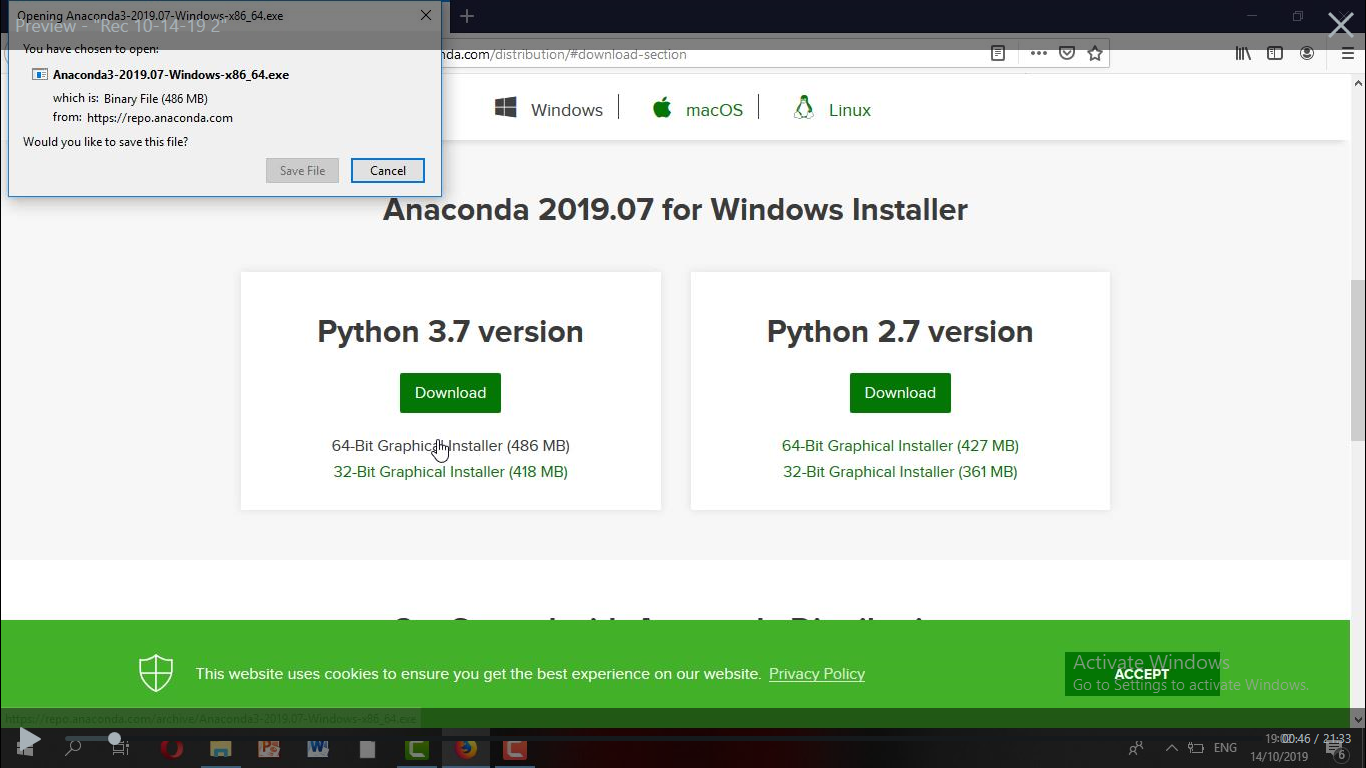
\includegraphics[width=4cm]{figure/3.png}
			\centering
			\caption{installation type}
			\end{figure}
		\item Pilih lokasi penyimpanan yang akan diinstal, lalu clik next.
			\begin{figure}[h]
			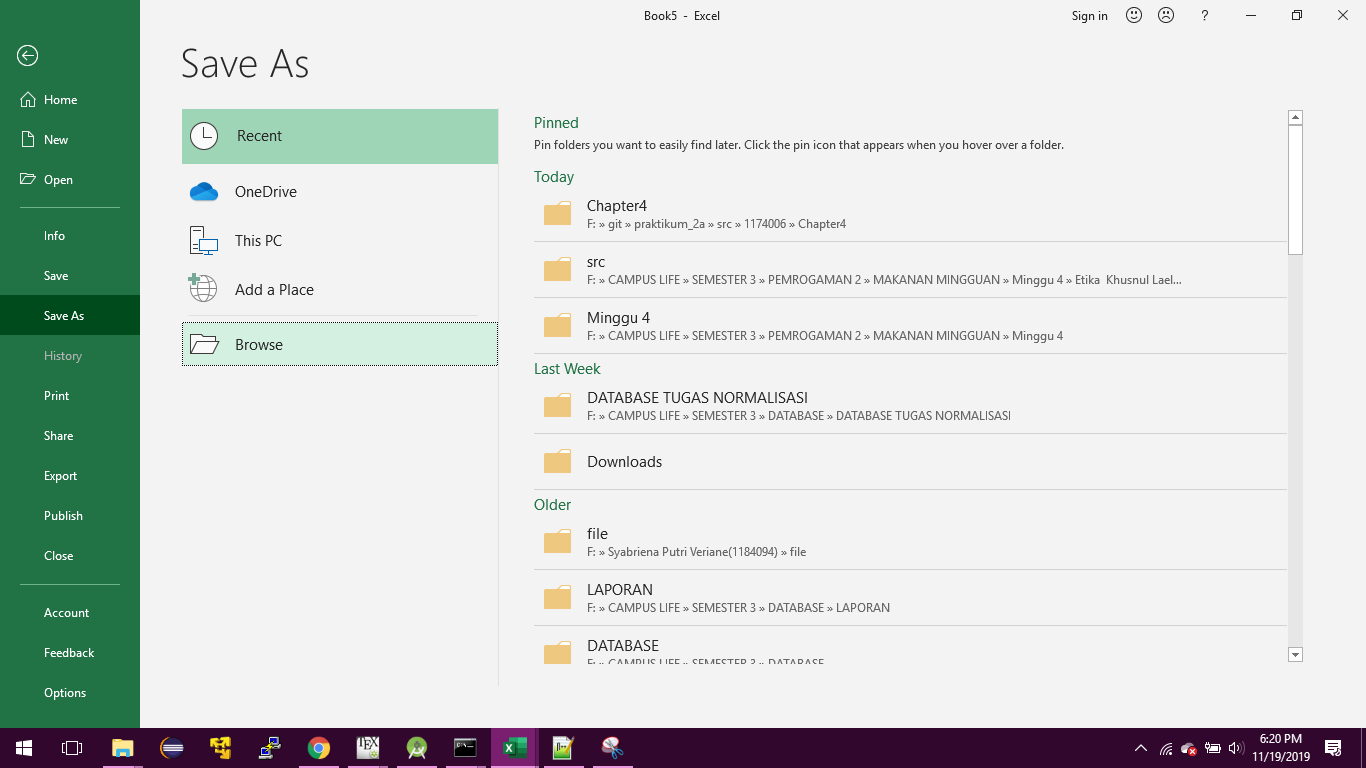
\includegraphics[width=4cm]{figure/4.png}
			\centering
			\caption{lokasi penyimpanan file anaconda}
			\end{figure}
		\item Ceklis bagian ADD Environtment to the Path, hal ini memungkinkan untuk menambahkan environtment anaconda ke dalam path yang ada dalam PC anda. Setelah itu klik next.
			\begin{figure}[h]
			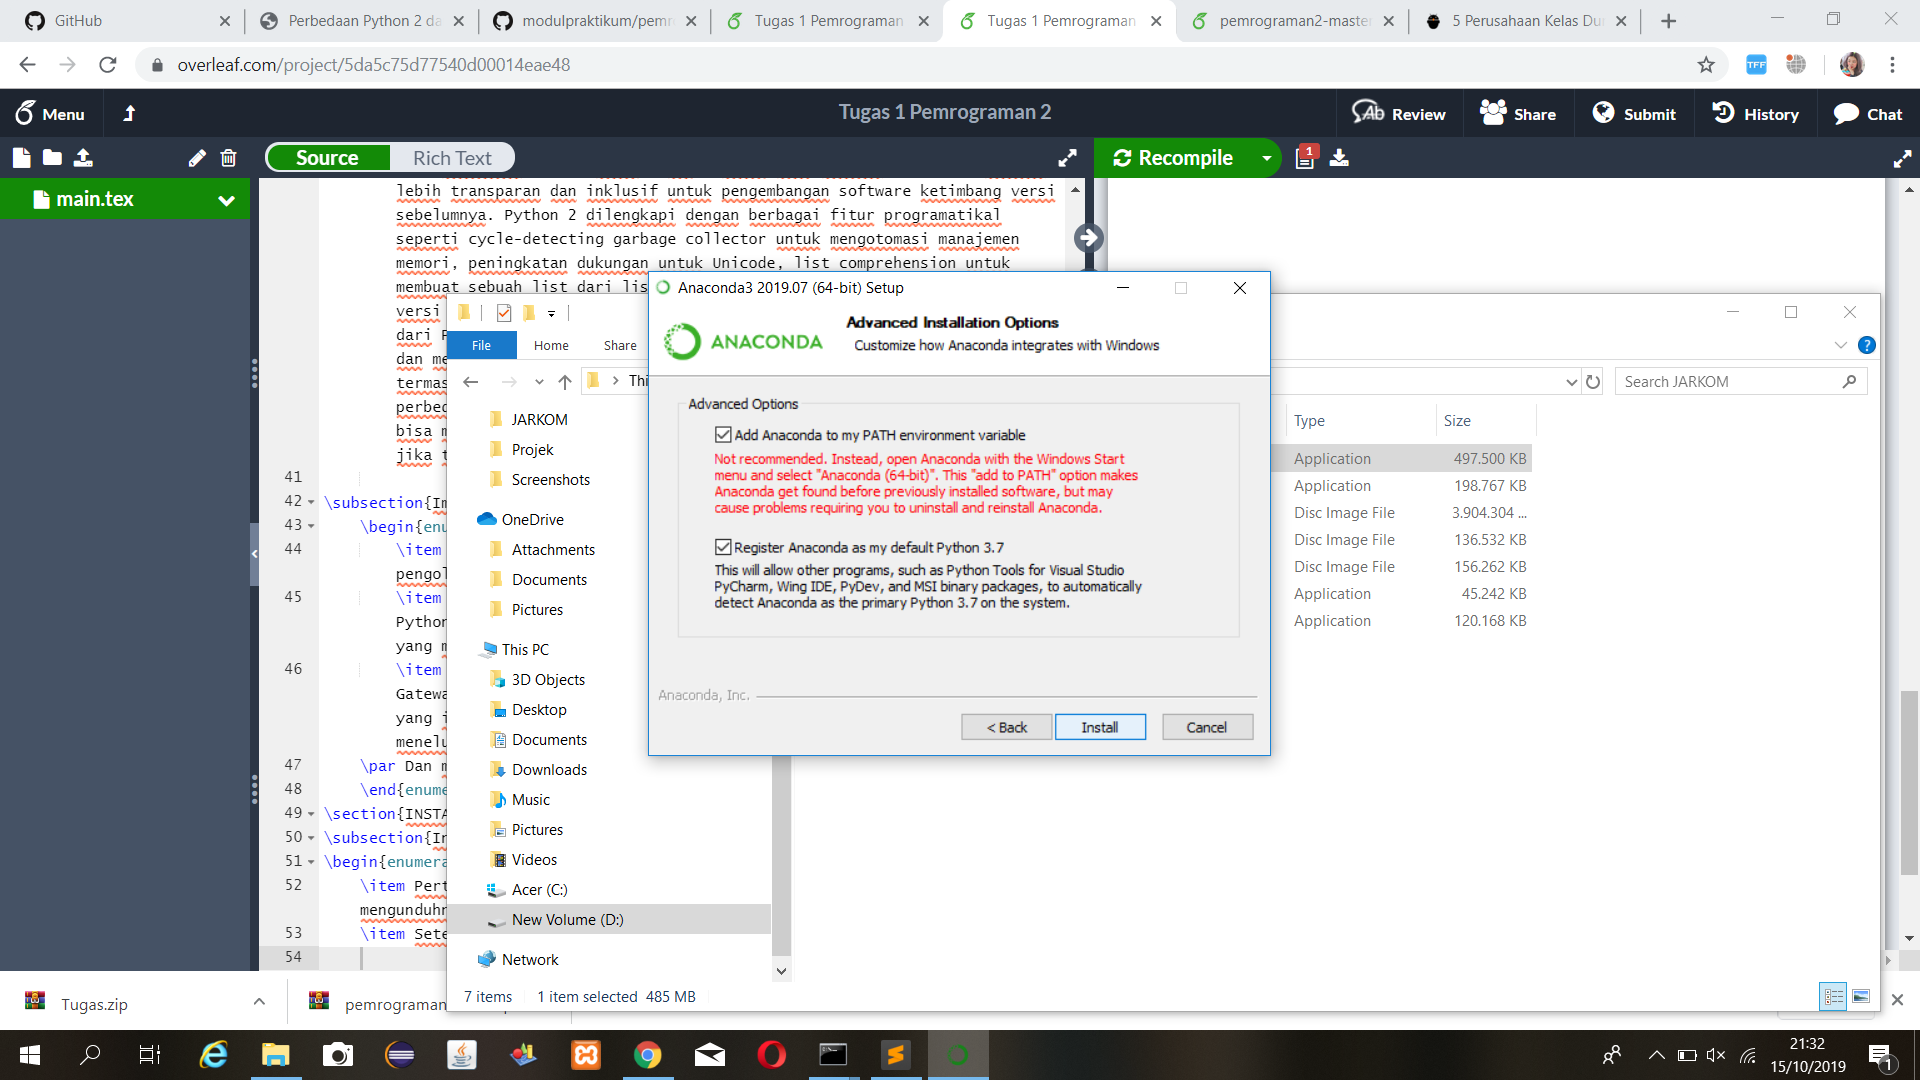
\includegraphics[width=4cm]{figure/5.png}
			\centering
			\caption{menambahkan path environtment}
			\end{figure}
		\item Tunggu instalan sampai selesai.
			\begin{figure}[h]
			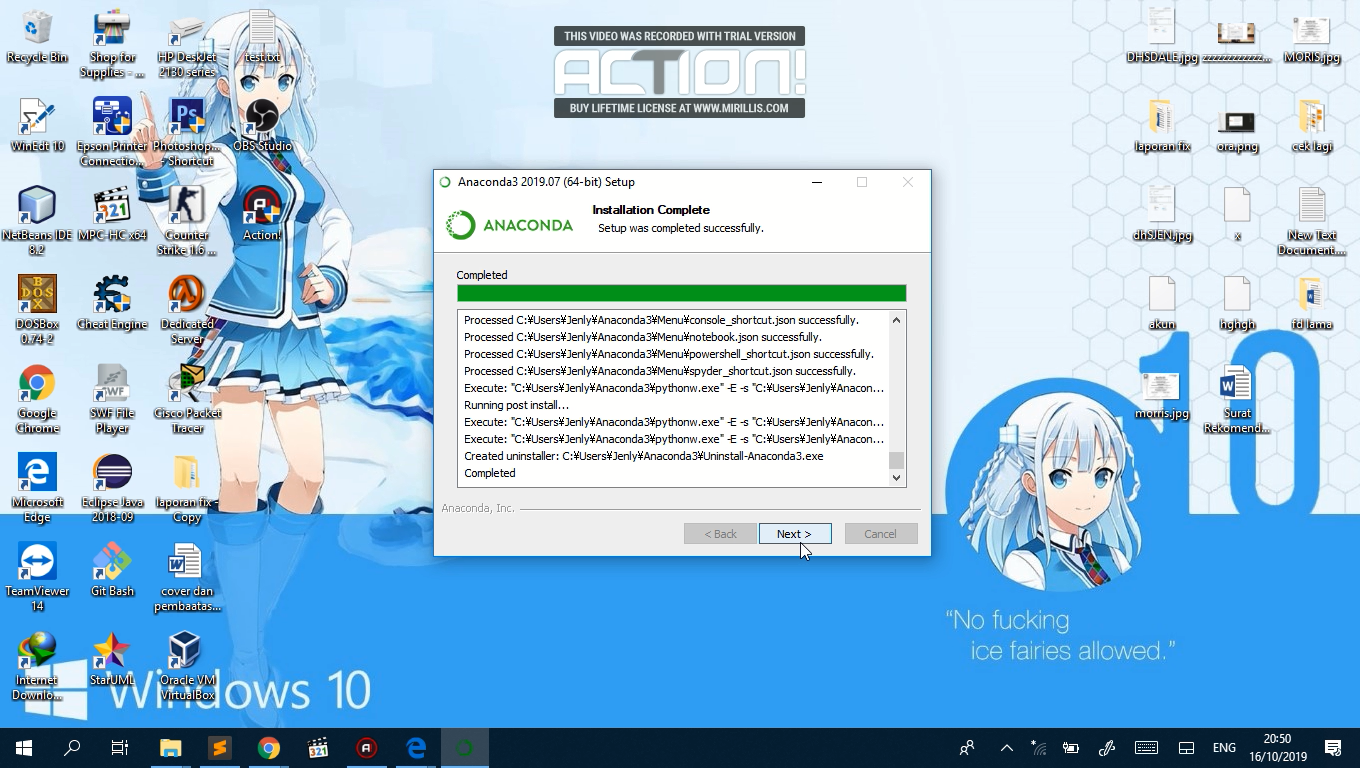
\includegraphics[width=4cm]{figure/7.png}
			\centering
			\caption{proses instalasi}
			\end{figure}
		\item Setelah Instal selesai, lau clik next sampai proses terakhir dan clik finish di akhir proses instal.
			\begin{figure}[h]
			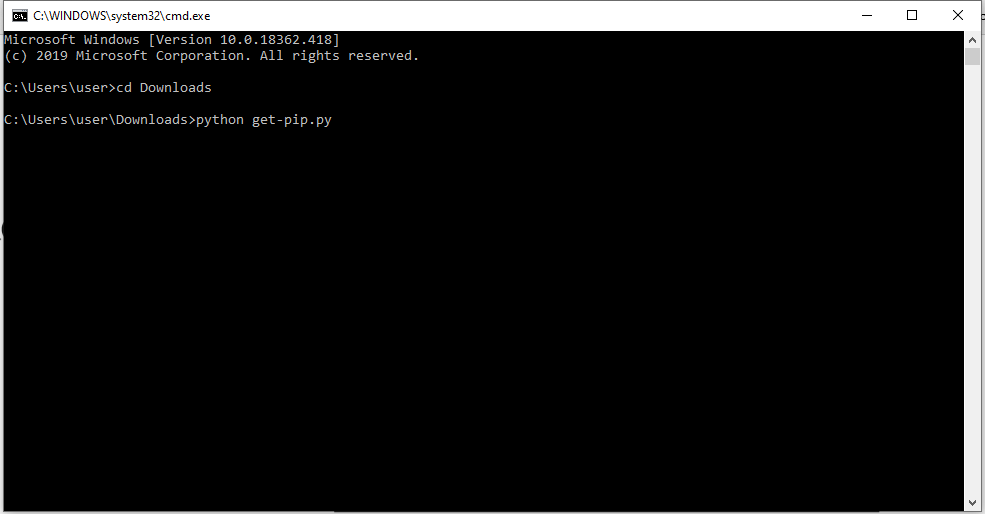
\includegraphics[width=4cm]{figure/8.png}
			\centering
			\caption{instalasi selesai}
			\end{figure}
		\item Click next.	
			\begin{figure}[h]
			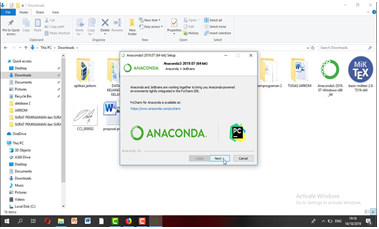
\includegraphics[width=4cm]{figure/9.png}
			\centering
			\caption{instalasi selesai 2}
			\end{figure}
		\item Click next lagi.	
			\begin{figure}[h]
			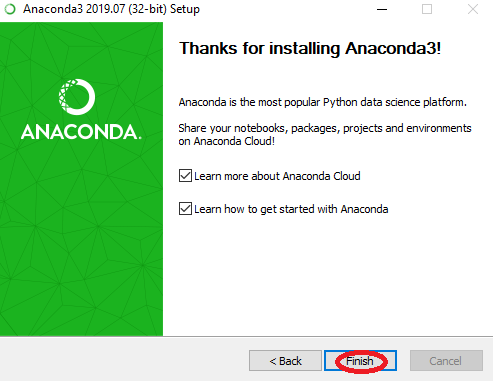
\includegraphics[width=4cm]{figure/10.png}
			\centering
			\caption{instalasi selesai 3}
			\end{figure}
		\item Lalu click finish.	
	\end{enumerate}

\section*{\textit{ Instalasi Pip }}
\begin{enumerate}
\item Buka Cmd (CommandPrompt)
\begin{figure}[h]
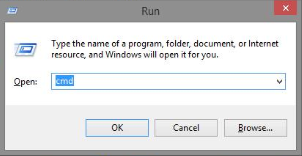
\includegraphics[width=4cm]{figure/pip1.png}
\centering
\caption{Buka Cmd}
\end{figure}
\item masuk kedalam direktori yang ada file pip nya.
\begin{figure}[h]
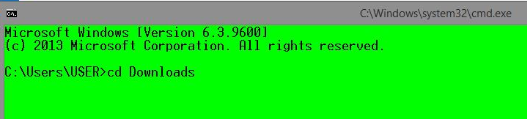
\includegraphics[width=4cm]{figure/pip2.png}
\centering
\caption{Masuk kedalam Direktori}
\end{figure}
\item Ketikan syntax untuk install pip nya
\begin{figure}[h]
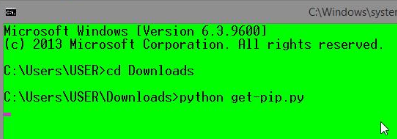
\includegraphics[width=4cm]{figure/pip3.png}
\centering
\caption{Mengetik Syntax}
\end{figure}
\item Jika sudah ada bacaan successfuly instaled, proses instalasi sudah selesai
\begin{figure}[h]
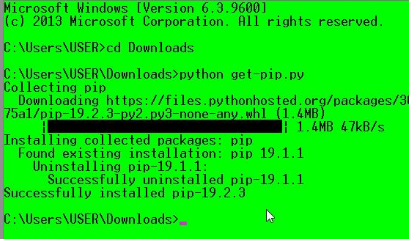
\includegraphics[width=4cm]{figure/pip4.png}
\centering
\caption{Selesai Install}
\end{figure}
\end{enumerate}

\section*{\textit{ Cara setting environment }}

\begin{enumerate}

\item Buka file exploler, lal click kanan di this pc, pilih properties
\begin{figure}[h]
\centering
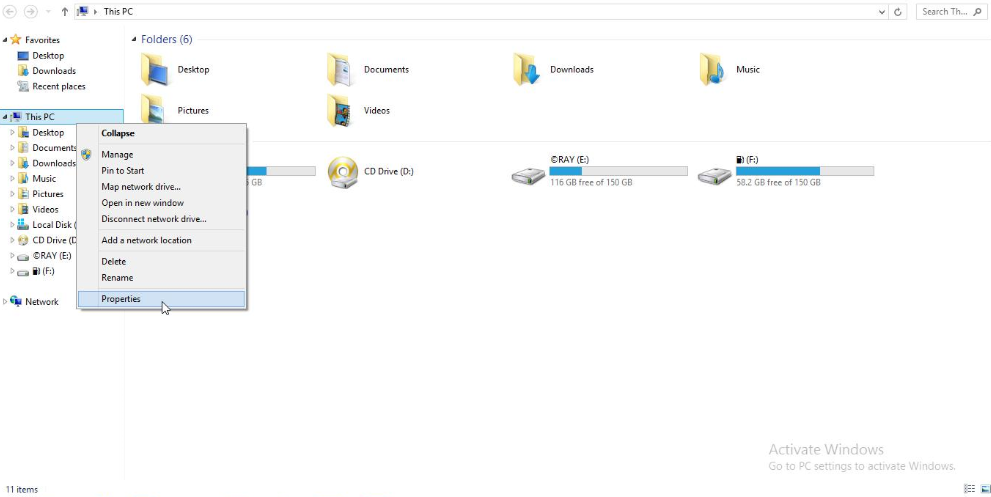
\includegraphics[scale=0.8]{figure/setting1.png}
\caption{membuka file exploler}
\end{figure}

\item Buka advance system settings
\begin{figure}[hb]
\centering
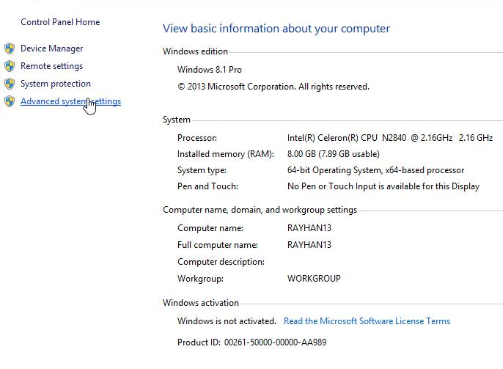
\includegraphics[scale=0.8]{figure/setting2.png}
\caption{membuka advance system}
\end{figure}

\item Click environment variables
\begin{figure}[hb]
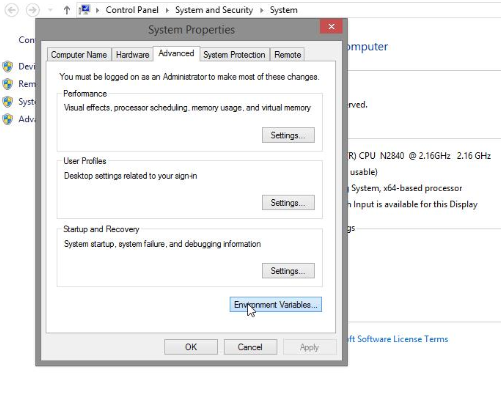
\includegraphics[width=4cm]{figure/setting3.png}
\centering
\caption{membuka environtment variables}
\end{figure}

\item Jika ingin mensetting pilih editt
\begin{figure}[h]
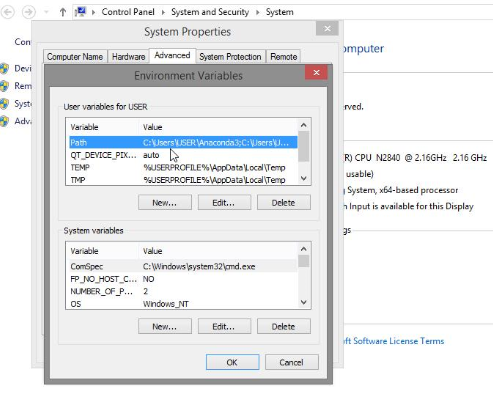
\includegraphics[width=4cm]{figure/setting4.png}
\centering
\caption{mensetting}
\end{figure}

\section*{\textit{ mencoba entrepreter/cli melakui terminal atau cmd windows }}

\begin{enumerate}

\item Buka Cmd
\begin{figure}[hb]
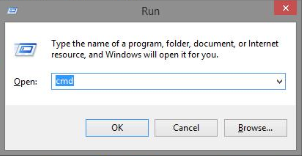
\includegraphics[width=4cm]{figure/interpreter1.png}
\centering
\caption{membuka Cmd}
\end{figure}

\item Menuliskan syntax
\begin{figure}[hb]
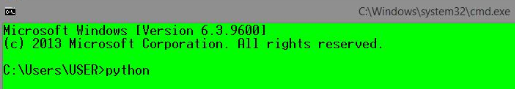
\includegraphics[width=4cm]{figure/interpreter2.png}
\centering
\caption{menuliskan syntax python}
\end{figure}

\item Menuliskan syntax
\begin{figure}[hb]
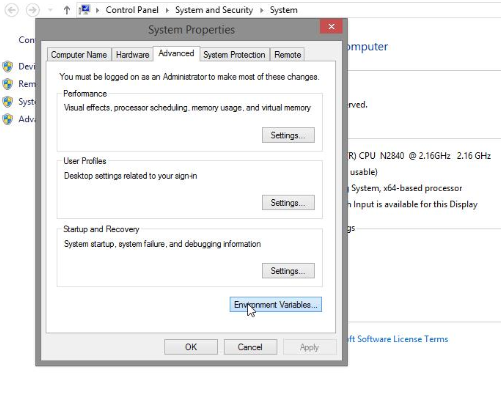
\includegraphics[width=4cm]{figure/setting3.png}
\centering
\caption{menuliskan syntax}
\end{figure}

\item melihat hasil syntax
\begin{figure}[hb]
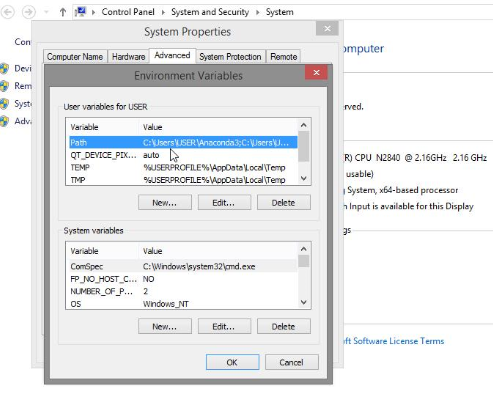
\includegraphics[width=4cm]{figure/setting4.png}
\centering
\caption{melihat hasil}
\end{figure}

\end{enumerate}

\section*{\textit{ Menjalankan dan mengupdate anaconda dan spyder }}

\begin{enumerate}

\item Buka aplikasi anaconda, lalu pilih environment.
\begin{figure}[hb]
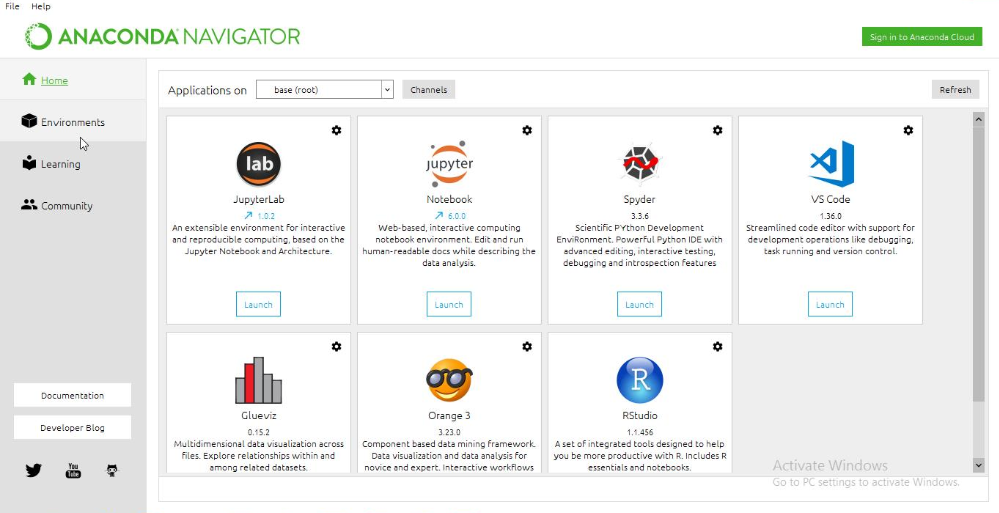
\includegraphics[width=4cm]{figure/update1.png}
\centering
\caption{membuka aplikasi}
\end{figure}

\item Menuliskan spyder di search package
\begin{figure}[hb]
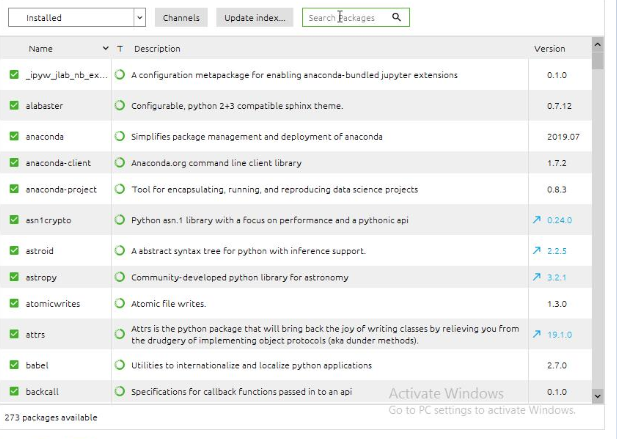
\includegraphics[width=4cm]{figure/update2.png}
\centering
\caption{search package}
\end{figure}

\item Click kanan pada tanda centang pada bacaan spyder, lalu pilih mark for specific version instalation.
\begin{figure}[hb]
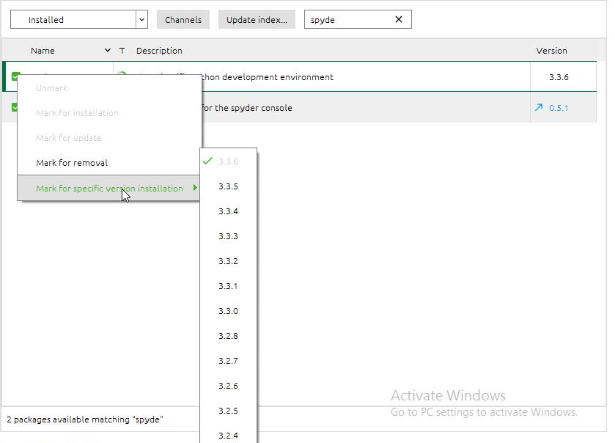
\includegraphics[width=4cm]{figure/update3.png}
\centering
\caption{memilih versi yang akan di install}
\end{figure}

\item Sama seperti yang tadi, search package yang akan di install lalu pilih versi yang akan di up.
\begin{figure}[hb]
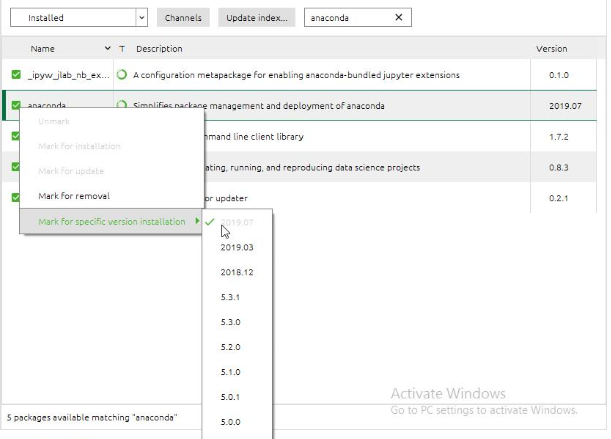
\includegraphics[width=4cm]{figure/update5.png}
\centering
\caption{mengupdate anaconda}
\end{figure}

\end{enumerate}

\section*{\textit{ Cara menjalankan Script hello word di spyder }}

\begin{enumerate}

\item Buka aplikasi spyder.
\begin{figure}[hb]
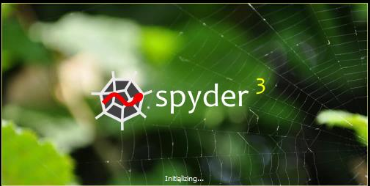
\includegraphics[width=4cm]{figure/pemakaian1.png}
\centering
\caption{membuka aplikasi}
\end{figure}

\item Menuliskan syntax 
\begin{figure}[hb]
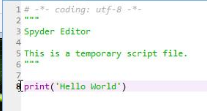
\includegraphics[width=4cm]{figure/pemakaian2.png}
\centering
\caption{Menuliskan syntax}
\end{figure}

\item Hasil syntax.
\begin{figure}[hb]
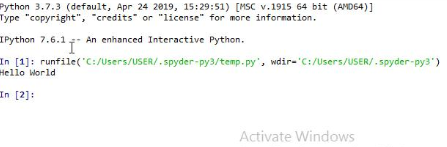
\includegraphics[width=4cm]{figure/pemakaian3.png}
\centering
\caption{Hasil syntax}
\end{figure}

\end{enumerate}

\section*{\textit{Cara menjalankan Script otomatis login aplikasi akademik dengan library selenium dan inputan user}}

\begin{enumerate}

\item Buka aplikasi spyder.
\begin{figure}[hb]
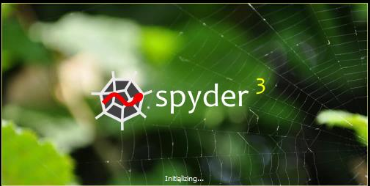
\includegraphics[width=4cm]{figure/pemakaian1.png}
\centering
\caption{membuka aplikasi}
\end{figure}

\item Menuliskan syntax 
\begin{figure}[hb]
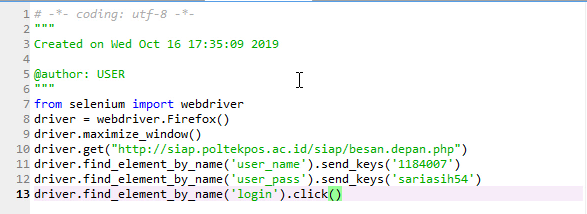
\includegraphics[width=4cm]{figure/login.png}
\centering
\caption{Menuliskan syntax}
\end{figure}

\item Hasil syntax.
\begin{figure}[hb]
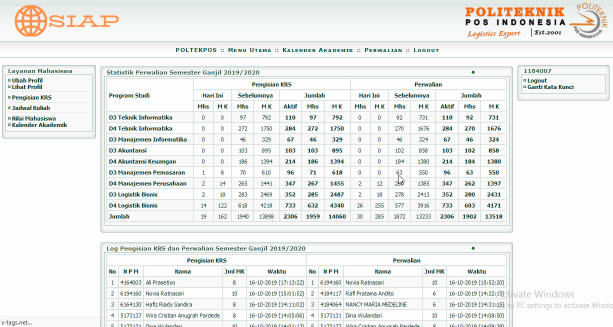
\includegraphics[width=4cm]{figure/login1.png}
\centering
\caption{Hasil syntax}
\end{figure}

\end{enumerate}


\section*{\textit{ Cara menjalankan Script otomatis login aplikasi akademik dengan library sele-
nium dan inputan user }}

\begin{enumerate}

\item Buka aplikasi spyder.
\begin{figure}[hb]
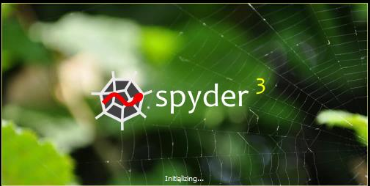
\includegraphics[width=4cm]{figure/pemakaian1.png}
\centering
\caption{membuka aplikasi}
\end{figure}

\item Menuliskan syntax 
\begin{figure}[hb]
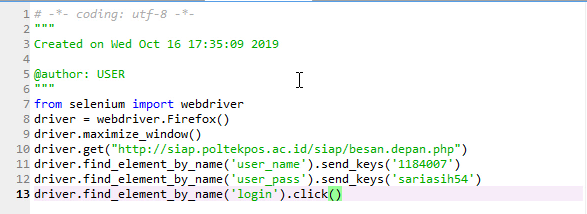
\includegraphics[width=4cm]{figure/login.png}
\centering
\caption{Menuliskan syntax}
\end{figure}

\item Hasil syntax.
\begin{figure}[hb]
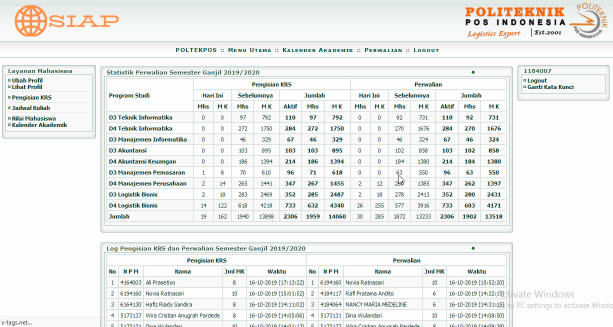
\includegraphics[width=4cm]{figure/login1.png}
\centering
\caption{Hasil syntax}
\end{figure}

\end{enumerate}

\section*{\textit{ Cara pemakaian variable explorer di spyder }}

\begin{enumerate}

\item Buka aplikasi spyder.
\begin{figure}[hb]
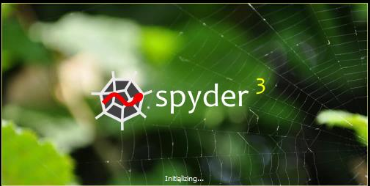
\includegraphics[width=4cm]{figure/pemakaian1.png}
\centering
\caption{membuka aplikasi}
\end{figure}

\item Menuliskan syntax 
\begin{figure}[hb]
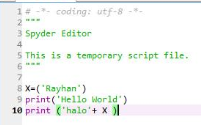
\includegraphics[width=4cm]{figure/pemakaian4.png}
\centering
\caption{Menuliskan syntax}
\end{figure}

\item Hasil syntax.menunjukan nama variable, type, dan value
\begin{figure}[hb]
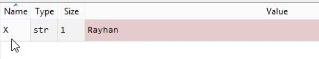
\includegraphics[width=4cm]{figure/pemakaian5.png}
\centering
\caption{Hasil syntax}
\end{figure}

\end{enumerate}




